\documentclass{eh-homework}

\usetikzlibrary{arrows.meta}

\begin{document}
    \begin{question}{1}
        Find the error term for the derivative approximation:
        \[
            f''(x_0) \approx \frac{2f(x_0 - h) - 3f(x_0) + f(x_0 + 2h)}{3h^2}.
        \]
    \end{question}
    \begin{question}{2}
        Find the error term for the quadrature method, and state its degree of precision.
        \[
            \int _{x_0}^{x_0 + 2h}f(x)\ dx \approx \frac{h}{2}\left[ 3f \left( x_0 + \frac{4}{3}h \right) + f(x_0) \right].
        \]
    \end{question}
    \begin{question}{3}
        Consider the integral \(\int _1^7 \cos (x^2)\ dx\)
        \begin{enumerate}[label=(\alph*)]
            \item Use the composite Simpson's rule to approximate the value of this integral using \(n=3\) intervals.
            \item Determine the number of intervals \(n\) needed to guarantee an error of at most \(10^{-4}\).
        \end{enumerate}
    \end{question}
    \begin{question}{4}
        Consider the IVP:
        \[
            2\dot y + y = t^4 + 1,\ y(1) = 2.
        \]
        Apply the second degree Taylor method with \(h = 0.5\) to this ODE to approximate \(y(2)\). Show the details in each step.
    \end{question}
    \begin{question}{5}
        Derive an ODE solver based on the stencil and corresponding integration formula.

        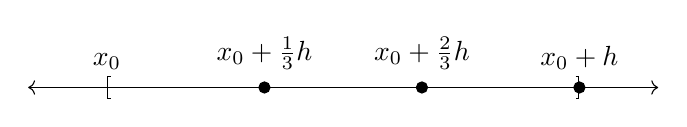
\begin{tikzpicture}
            \draw[<->] (-1, 0) -- (7, 0);
            \draw[{Bracket[width=3mm]}-{Bracket[width=3mm]}] (0, 0) -- (6,0);
            \node[above] at (0, 0.1) {\(x_0\)};
            \foreach \x/\val in {2/\(x_0 + \frac{1}{3}h\), 4/\(x_0 + \frac{2}{3}h\), 6/\(x_0 + h\)} {
                \draw[fill] (\x, 0) circle (2pt);
                \node[above] at (\x, 0.1) {\val};
            }

        \end{tikzpicture}
        Formula: \(\frac{h}{4}\left( 3f \left( x_0 + \frac{1}{3}h \right) + f(x_0 + h) \right) + O (h^4)\) 
    \end{question}
\end{document}